\documentclass[a4paper,titlepage]{article}
\usepackage[utf8]{inputenc}
\usepackage{fullpage}
\usepackage{indentfirst}
\usepackage[per-mode=symbol]{siunitx}
\usepackage{listings}
\usepackage{graphicx}
\usepackage{color}
\usepackage{amsmath}
\usepackage{array}
\usepackage[hidelinks]{hyperref}
\usepackage[format=plain,font=it]{caption}
\usepackage{subcaption}
\usepackage{standalone}
\usepackage[nottoc]{tocbibind}
\usepackage[noabbrev,capitalize,nameinlink]{cleveref}
\usepackage{listings}
\usepackage{titlesec}
\usepackage{minted}
\usepackage{booktabs}
\usepackage{csvsimple}
\usepackage{siunitx}
\usepackage[super]{nth}
\usepackage[titletoc]{appendix}
\usepackage{todonotes}
\usepackage{mathtools}
\usepackage{relsize}

% Custom commands
\newcommand\numberthis{\addtocounter{equation}{1}\tag{\theequation}}
\newcommand{\code}[1]{\texttt{#1}}
\newcolumntype{P}[1]{>{\centering\arraybackslash}p{#1}}

\setminted{linenos,breaklines,fontsize=auto}

%\titleformat*{\section}{\normalsize\bfseries}
%\titleformat*{\subsection}{\small\bfseries}
\renewcommand{\thesubsection}{\thesection.\alph{subsection}}
\providecommand*{\listingautorefname}{Listing}
\newcommand*{\Appendixautorefname}{Appendix}
%\crefname{appendix}{Appendix}{Appendices}
%\def\appendixname{Appendix}


%opening
\title{\textbf{ECSE 543 \\ Assignment 3}}
\author{Sean Stappas \\ 260639512}
\date{December \nth{7}, 2017}

\begin{document}
	\sloppy
	\maketitle
	
	\tableofcontents
	
	
	\twocolumn
	
	\section*{Introduction}
	The code for this assignment was created in Python 2.7 and can be seen in \autoref{appendix:code}. To perform the required tasks in this assignment, the \mintinline{python}{Matrix} class from Assignment 1 was used, with useful methods such as add, multiply, transpose, etc. This package can be seen in the \mintinline{python}{matrices.py} file shown in \autoref{lst:matrices}. The only packages used that are not built-in are those for creating the plots for this report, i.e., \mintinline{python}{matplotlib} for plotting. The structure of the rest of the code will be discussed as appropriate for each question. Output logs of the program are provided in \autoref{appendix:logs}.
	
	
	\section{BH Interpolation}
	The source code for the Question 1 program can be seen in the \mintinline{python}{q1.py} file shown in \cref{lst:q1}.
	
	\subsection{Lagrange Polynomials}
	To interpolate $n=6$ points of a function $y(x)$, six \nth{5}-order Lagrange polynomials are needed. Each of these polynomials $L_j$ is given by \cref{eq:lagrange_polynomial}, where each $F_j$ is given by \cref{eq:lagrange_f}.
	
	\begin{equation} \label{eq:lagrange_polynomial}
		L_j(x) = \frac{F_j(x)}{F_j(x_j)}
	\end{equation}
	
	\begin{equation} \label{eq:lagrange_f}
		F_j(x) = \smashoperator{\prod\limits_{r=1 \ldots n, r \neq j}} (x - x_r)
	\end{equation}
	
	The interpolation $\tilde{y}(x)$ of $y(x)$ is then given by \cref{eq:lagrange_interpolation}.
	
	\begin{equation} \label{eq:lagrange_interpolation}
		\tilde{y}(x) = \sum_{j=1}^{n} y(x_j) L_j(x)
	\end{equation}
	
	To ease the handling of these polynomials, a \code{Polynomial} class was created, with useful methods like \code{add}, \code{multiply} and \code{evaluate}. This class can be found in the \code{polynomial.py} file shown in \cref{lst:polynomial} and the associated tests can be found in the \code{polynomial\_test.py} file shown in \cref{lst:test_polynomial}.
	
	The code evaluating the polynomials in \cref{eq:lagrange_f,eq:lagrange_polynomial,eq:lagrange_interpolation} for interpolation can be found in the \code{lagrange.py} file shown in \cref{lst:lagrange}. The associated tests are in the \code{test\_lagrange.py} file shown in \cref{lst:test_lagrange}.
	
	The interpolation for the first 6 points of the $B$-$H$ curve is evaluated in \code{q1.py} shown in \cref{lst:q1}, with output logged in \cref{lst:q1_log}. The generated plot can be seen in \cref{fig:q1a}. It can be seen that the interpolation passes through all the data points, as expected. The curve is also relatively smooth, and should be a good approximation of the $B$-$H$ curve over that range.
	
	\begin{figure}[!htb]
		\centering
		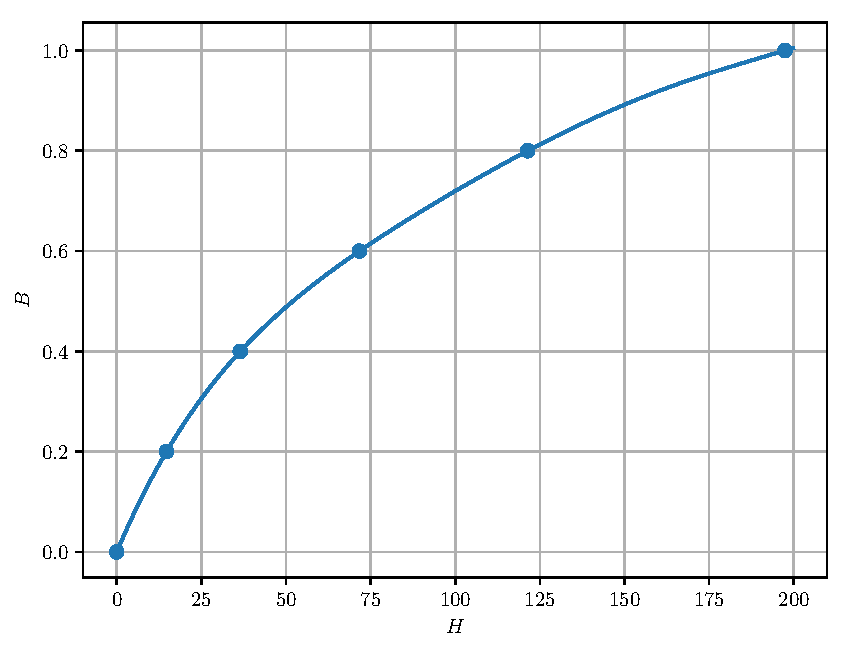
\includegraphics[width=\columnwidth]{plots/q1a.pdf}
		\caption
		{Lagrange interpolation of the first 6 points ($B = 0.0, 0.2, 0.4, 0.6, 0.8, 1.0$) in the $B$-$H$ curve. The points are from the table and the curve is interpolated.}
		\label{fig:q1a}
	\end{figure}
	
	\subsection{Full-Domain Interpolation}	
	
	The interpolation for the given six points is computed in \code{q1.py} shown in \cref{lst:q1} with output in \cref{lst:q1_log}. The generated plot can be seen in \cref{fig:q1b}. The curve passes through all the given points, but is clearly not plausible. It has the characteristic ``wiggles'' seen when using full-domain Lagrange polynomials over a wide range. It even shows negative $B$ values, which do not match the actual values in between the chosen points.
	
	\begin{figure}[!htb]
		\centering
		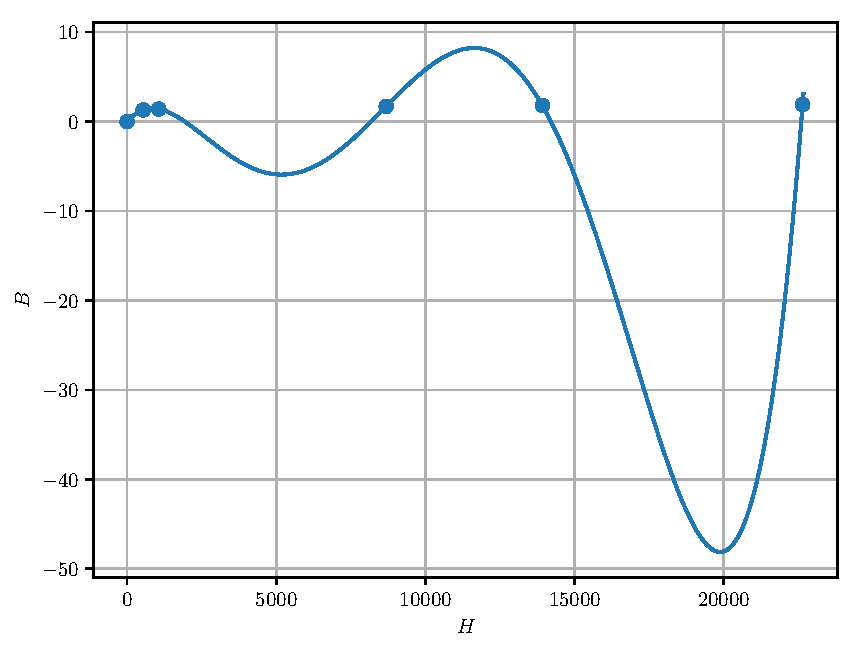
\includegraphics[width=\columnwidth]{plots/q1b.pdf}
		\caption
		{Lagrange interpolation of 6 points ($B = 0.0, 1.3, 1.4, 1.7, 1.8, 1.9$) in the $B$-$H$ curve. The points are from the table and the curve is interpolated.}
		\label{fig:q1b}
	\end{figure}
	
	\subsection{Cubic Hermite Polynomials} \label{sec:cubic_hermite}
	The slopes at each of the 6 points can be approximated by the slope of the straight line passing through the two adjacent points, i.e., the point immediately before and the point after the point of interest. For the boundary points of \SI{0}{\tesla} and \SI{1.9}{\tesla}, the slope of the line formed by the point and one adjacent point can be used.
	
	\section{Magnetic Circuit}
	The source code for the Question 2 program can be seen in the \mintinline{python}{q2.py} file shown in \cref{lst:q2}.
	
	\subsection{Flux Equation}
	The magnetic analog of KVL can be seen in \cref{eq:magnetic_kvl}.

	\begin{equation} \label{eq:magnetic_kvl}
		(\mathcal{R}_a + \mathcal{R}_c) \psi = \mathcal{F}
	\end{equation}
	where $\mathcal{R}_a$ is the reluctance of the air gap, $\mathcal{R}_c$ is the reluctance of the coil, and $\mathcal{F}$ is the magnetomotive force. Plugging in the relevant variables from the problem, we obtain \cref{eq:magnetic_kvl_plug}.

	\begin{equation} \label{eq:magnetic_kvl_plug}
		\left( \frac{L_a}{A \mu_o} + \frac{L_c}{A \mu_c(\psi)} \right) \psi - NI = 0
	\end{equation}
	where $\mu_c(\psi)$ is a function of $\psi$ given by \cref{eq:mu}.
	
	\begin{equation} \label{eq:mu}
		\mu_c(\psi) = \frac{B(\psi)}{H(\psi)} = \frac{\psi}{A H(\psi)}
	\end{equation}
	
	Plugging \cref{eq:mu} into \cref{eq:magnetic_kvl_plug}, we obtain \cref{eq:magnetic_kvl_plug_2}.
	
	\begin{equation} \label{eq:magnetic_kvl_plug_2}
		\left( \frac{L_a}{A \mu_o} + \frac{L_c H(\psi)}{\psi} \right) \psi - NI = 0
	\end{equation}
	
	Simplifying the terms, we obtain \cref{eq:flux}.
	
	\begin{equation} \label{eq:flux}
		f(\psi) = \frac{L_a \psi}{A \mu_o} + L_c H(\psi) - NI = 0
	\end{equation}
	
	Finally, if we plug in the values from the question, we obtain \cref{eq:flux_plug}, where the coefficients of the terms are calculated in the \mintinline{python}{q2.py} script shown in \cref{lst:q1}.
	
	\begin{equation} \label{eq:flux_plug}
		\input{latex/flux_equation.txt}
	\end{equation}
	
	In \cref{eq:flux_plug}, $H(\psi)$ can be calculated for a given $\psi$ by first finding $B = \psi / A$, and then using the $B$-$H$ curve to find $H$.
	
	\subsection{Newton-Raphson}
	
	To perform the Newton-Raphson update, the derivative $f'$ of $f$ will be needed. This can be seen in \cref{eq:flux_derivative}, where the $1/A$ term comes from the fact that $B(\psi) = \psi / A$ and $H(\psi) = H(B(\psi)) = H(\psi / A)$.
	
	\begin{equation} \label{eq:flux_derivative}
		\begin{split}
			f'(\psi) &= \SI{3.979e7}{} + \frac{0.3H'(\psi)}{A} \\
			&= \SI{3.979e7}{} + 3000 H'
		\end{split}
	\end{equation}
	
	In \cref{eq:flux_derivative}, the derivative $H'$ of $H$ can be estimated using the slope between each of the points given in the $B$-$H$ table of Question 1.	The slope interpolation code is in the \code{slope\_interpolation.py} script shown in \cref{lst:slope_interpolation}.
	
	A piecewise-linear interpolation of the data in the $B$-$H$ table is needed. This can easily be obtained using the Lagrange polynomial program created for Question 1. Here, we simply need to interpolate 2 points in every sub-domain using \nth{1}-order Lagrange polynomials. We will also need to interpolate $H$ as a function of $B$ to evaluate \cref{eq:flux_plug}, unlike in Question 1. The linear interpolation code is in the \code{piecewise\_linear.py} script shown in \cref{lst:piecewise_linear}. The generated piecewise-linear interpolation fits the $B$-$H$ points, as can be seen in \cref{fig:q2b}.
	
	\begin{figure}[!htb]
		\centering
		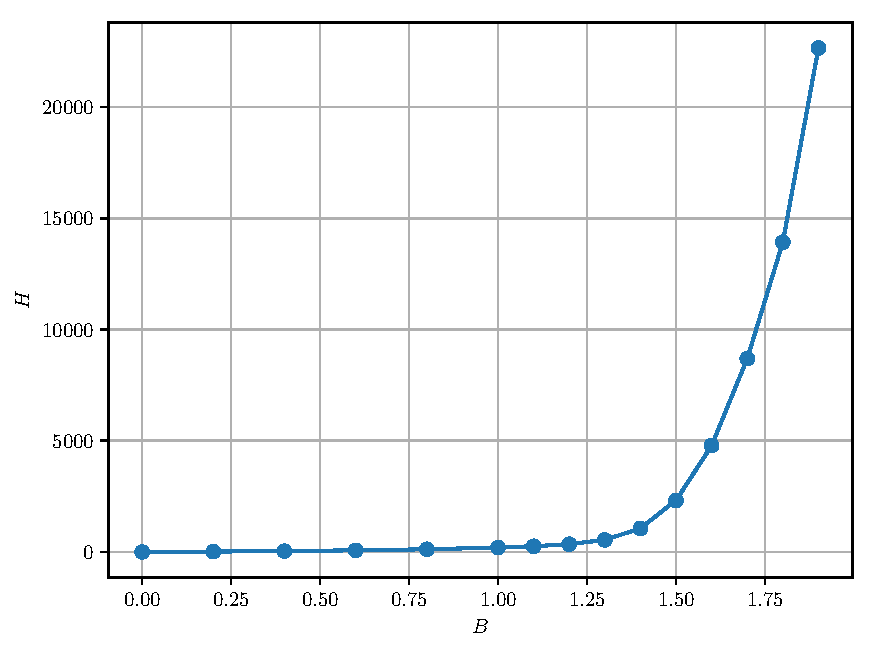
\includegraphics[width=\columnwidth]{plots/q2b.pdf}
		\caption
		{Piecewise-linear interpolation of the $H$-$B$ curve.}
		\label{fig:q2b}
	\end{figure}
	
	With $f$ given by \cref{eq:flux_plug} and $f'$ given by \cref{eq:flux_derivative}, the Newton-Raphson update equation for the flux $\psi$ is given by \cref{eq:newton_raphson}.
	
	\begin{equation} \label{eq:newton_raphson}
		\psi^{(k+1)} \leftarrow \psi^{(k)} - \frac{f^{(k)}}{{f'}^{(k)}}
	\end{equation}
	
	The code performing the Newton-Raphson update is in \code{newton\_raphson.py} and can be seen in \cref{lst:newton_raphson}. The executing program is in \code{q2.py} shown in \cref{lst:q2}, with associated output in \cref{lst:q2_log}. The program takes 3 steps to solve for a flux of approximately $\psi = \SI{161.269}{\micro\weber}$.
	
	\subsection{Successive Substitution}
	
	
	\section{Diode Circuit}
	The source code for the Question 3 program can be seen in the \mintinline{python}{q3.py} file shown in \cref{lst:q3}.
	
	\subsection{Voltage Equations}
	The current-voltage relationship for a diode is given by \cref{eq:diode_iv}.
	
	\begin{equation} \label{eq:diode_iv}
		I = I_s \left( \exp\left[{\frac{qv}{kT}}\right] - 1\right)
	\end{equation}
	
	Let the nodal voltage at the anode of the A diode be denoted by $v_A$ and that of the B diode by $v_B$. Let the current through the circuit be denoted by $I$. The diode equations for A and B can be seen in \cref{eq:diode_A,eq:diode_B}.
	
	\begin{equation} \label{eq:diode_A}
		I = I_{sA} \left( \exp\left[{\frac{q(v_A - v_B)}{kT}}\right] - 1\right)
	\end{equation}
	
	\begin{equation} \label{eq:diode_B}
		I = I_{sB} \left( \exp\left[{\frac{qv_B}{kT}}\right] - 1\right)
	\end{equation}
	
	By KVL, we also have \cref{eq:diode_kvl}, relating $V_A$ and $I$.
	
	\begin{equation} \label{eq:diode_kvl}
		I = \frac{E - v_A}{R}
	\end{equation}
	
	Equating \cref{eq:diode_kvl,eq:diode_A}, we obtain the nonlinear equation for $v_A$, shown in \cref{eq:diode_voltage_A}.
	
	\begin{equation} \label{eq:diode_voltage_A}
	\begin{split}
		&f_A(v_A, v_B) \\
		& = v_A + R I_{sA} \left( \exp\left[{\frac{q(v_A - v_B)}{kT}}\right] - 1\right) - E \\
		& = 0
	\end{split}
	\end{equation}
	
	Equating \cref{eq:diode_A,eq:diode_B}, we obtain the nonlinear equation for $v_B$, shown in \cref{eq:diode_voltage_B}.
	
	\begin{align} \label{eq:diode_voltage_B}
	\begin{split}
		f_B(v_A, v_B) &= I_{sA} \left( \exp\left[{\frac{q(v_A - v_B)}{kT}}\right] - 1\right)\\
		&- I_{sB} \left( \exp\left[{\frac{qv_B}{kT}}\right] - 1\right) = 0
	\end{split}
	\end{align}
	
	The total system of equations can then be expressed by \cref{eq:f_system}.
	
	\begin{equation} \label{eq:f_system}
		\mathbf{f}(\mathbf{v_n}) = 
		\begin{bmatrix}
		f_A(v_A, v_B) \\
		f_B(v_A, v_B)
		\end{bmatrix}
		= \mathbf{0}
	\end{equation}
	
	
	\subsection{Newton-Raphson}
	
	To find an expression for the Jacobian matrix \textbf{F}, we must first find expressions for all the partials of $f_A$ and $f_B$. These are shown in \cref{eq:jacobian_11,eq:jacobian_12,eq:jacobian_21,eq:jacobian_22}.
	
	\begin{equation} \label{eq:jacobian_11}
		\frac{\partial f_A}{\partial v_A} = 1 + R I_{sA} \left( \exp\left[{\frac{q(v_A - v_B)}{kT}}\right]\frac{q}{kT}\right)
	\end{equation}
	
	\begin{equation} \label{eq:jacobian_12}
		\frac{\partial f_A}{\partial v_B} = - R I_{sA} \left( \exp\left[{\frac{q(v_A - v_B)}{kT}}\right]\frac{q}{kT}\right)
	\end{equation}
	
	\begin{equation} \label{eq:jacobian_21}
		\frac{\partial f_B}{\partial v_A} = I_{sA} \left( \exp\left[{\frac{q(v_A - v_B)}{kT}}\right]\frac{q}{kT}\right)
	\end{equation}
	
	\begin{equation} \label{eq:jacobian_22}
	\begin{split}
		\frac{\partial f_B}{\partial v_B} = &-I_{sA} \left( \exp\left[{\frac{q(v_A - v_B)}{kT}}\right]\frac{q}{kT}\right) \\
		&- I_{sB} \left( \exp\left[{\frac{qv_B}{kT}}\right]\frac{q}{kT}\right)
	\end{split}
	\end{equation}
	
	With these equations, the Jacobian matrix \textbf{F} is given by \cref{eq:jacobian}.
	
	\begin{equation} \label{eq:jacobian}
		\textbf{F} = 
		\begin{bmatrix}
		\dfrac{\partial f_A}{\partial v_A} & \dfrac{\partial f_A}{\partial v_B} \\[2ex]
		\dfrac{\partial f_B}{\partial v_A} & \dfrac{\partial f_B}{\partial v_B}
		\end{bmatrix}
	\end{equation}
	
	With this information, we can apply the Newton-Raphson update in matrix form, shown in \cref{eq:newton_raphson_matrix}.
	
	\begin{equation} \label{eq:newton_raphson_matrix}
		\mathbf{v_n}^{(k + 1)} \leftarrow \mathbf{v_n}^{(k)} - (\mathbf{F}^{(k)})^{-1} \mathbf{f}^{(k)}
	\end{equation}
	
	The code performing this update is in the \code{newton\_raphson\_matrix.py} script and can be seen in \cref{lst:newton_raphson_matrix}. The initial guess is $v_A=\SI{0}{\volt}$ and $v_B=\SI{0}{\volt}$. The program terminates when $\|\mathbf{f}\| / \|\mathbf{f_0}\|$ is less than some $\epsilon$, as shown in \cref{eq:newton_raphson_matrix_error}. The chosen value of $\epsilon$ is \SI{1e-9}{}.
	
	\begin{equation} \label{eq:newton_raphson_matrix_error}
		\frac{\|\mathbf{f}\|}{\|\mathbf{f_0}\|} < \epsilon
	\end{equation}
	
	The code is executed in the \code{q3.py} script shown in \cref{lst:q3}, with output shown in \cref{lst:q3_log}. The final solved voltage values are \SI{198.134}{\milli\volt} for $v_A$ and \SI{90.571}{\milli\volt} for $v_B$.
	
	
	\begin{table}[!htb]
		\centering
		\caption{Node voltages and \textbf{f} values at every iteration of Newton-Raphson.}
		\begin{tabular}{c | c | c}
			$v_A$ (mV) & $v_B$ (mV) & $\|\mathbf{f}\| / \|\mathbf{f_0}\|$ \\ \hline
			\input{latex/q3.txt}
		\end{tabular}
		\label{table:q3}
	\end{table}
	
	\section{Function Integration}
	The source code for the Question 4 program can be seen in the \mintinline{python}{q4.py} file shown in \cref{lst:q4}.
	
	\subsection{Cosine Integration}
	
	The integral $I$ to be solved by Gauss-Legendre integration is shown in \cref{eq:fx_integral}.
	
	\begin{equation} \label{eq:fx_integral}
		I = \int\limits_{x_1}^{x_2} f(x) dx 
	\end{equation}
	
	To use Gauss-Legendre integration over N equal segments, the $[x_1, x_2]$ range of $x$ must be mapped to N intervals of size $h$, with each interval $i$ having a center point $x_{0_i}$, with $x_i$ ranging from $x_{0_i} - h/2$ to $x_{0_i} + h/2$. Each of these intervals must be mapped to a $[-1, 1]$ range for $\zeta_i$. This mapping between $x_i$ and $\zeta_i$ over an interval is given by \cref{eq:x_zeta}.
	
	\begin{equation} \label{eq:x_zeta}
		x_i = x_{0_i} + \frac{h}{2} \zeta_i
	\end{equation}
	
	The integral transformation from $x$ to $\zeta$ over an interval $i$ is then given by \cref{eq:x_to_zeta_integral}.
	
	\begin{equation} \label{eq:x_to_zeta_integral}
	\begin{split}
			I_i &= \smashoperator{\int\limits_{x_{0_i} - h/2}^{x_{0_i} + h/2}} f(x_i) dx_i \\
			 &= \frac{h}{2} \int\limits_{-1}^{1} f \left[x_{0_i} + \frac{h}{2} \zeta_i\right] d\zeta_i
	\end{split}
	\end{equation}
	
	The one-point Gauss-Legendre approximation can then be applied for each interval, as shown in \cref{eq:one_point_interval}, where $w_0 = 2$.
	
	\begin{equation} \label{eq:one_point_interval}
		\begin{split}
			I_i &= \frac{h}{2} \int\limits_{-1}^{1} f \left[x_{0_i} + \frac{h}{2} \zeta_i\right] d\zeta_i \\
			&= \frac{h}{2} w_0 f(x_{0_i}) \\
			&= h f(x_{0_i})
		\end{split}
	\end{equation}
	
	The equation approximating $I$ is then given by \cref{eq:total_integral}.
	
	\begin{equation} \label{eq:total_integral}
		\begin{split}
				I &\approx \sum_{i=0}^{N-1} I_i \\
				&= \sum_{i=0}^{N-1} h f(x_{0_i}) \\
				&= h \sum_{i=0}^{N-1} f(x_{0_i})
		\end{split}
	\end{equation}
	
	To summarize, to solve an integral of the form shown in \cref{eq:fx_integral} with one-point Gauss-Legendre integration over N intervals, we simply need the width $h$ of each interval and the value $f(x_{0_i})$ of the function $f$ at the midpoint of every interval.
	
	In the context of this question, $x_1 = 0$ and $x_2 = 1$. The width of each interval is $h = 1/N$ and the midpoint of each interval is $x_{0_i} = 1/(2N) + i/N$. This yields the equation shown in \cref{eq:context_total_integral}.
	
	\begin{equation} \label{eq:context_total_integral}
		\begin{split}
			I &= \int\limits_{0}^{1} f(x) dx  \\
			&\approx \frac{1}{N} \sum_{i=0}^{N-1} f\left[ \frac{1}{N} \left(i + \frac{1}{2} \right) \right] \\
		\end{split}
	\end{equation}
	
	The code executing \cref{eq:context_total_integral} for arbitrary $f(x)$ can be seen in the \code{gauss\_legendre.py} script shown in \cref{lst:gauss_legendre}.
	
	If we use the fact that $f(x) = \cos x$ as well for this question, we obtain \cref{eq:cos_total_integral}.
	
	\begin{equation} \label{eq:cos_total_integral}
		I \approx \frac{1}{N} \sum_{i=0}^{N-1} \cos \left[ \frac{1}{N} \left(i + \frac{1}{2} \right) \right]
	\end{equation}
	
	To evaluate the estimation, it can be compared to actual value of the integral, which is given by \cref{eq:cos_actual_integral}.
	
	\begin{equation} \label{eq:cos_actual_integral}
		\int\limits_{0}^{1} \cos x dx = \sin 1 - \sin 0 = \sin 1 \approx 0.841
	\end{equation}
	
	The equation for the absolute error used is shown in \cref{eq:error}, where $I_{actual}$ is the actual value of the integral, and $I_{approx}$ is the approximate value computed by Gauss-Legendre integration.
	
	\begin{equation} \label{eq:error}
		E = | I_{actual}  - I_{approx}|
	\end{equation}
	
 	The integral of $\cos x$ is computed in the \code{q4.py} script shown in \cref{lst:q4}, with output shown in \cref{lst:q4_log}. The logarithmic plot of the error versus N can be seen in \cref{fig:q4a}. The straight-line slope of the plot is indicative of the fact that first-order Gauss-Legendre integration was used.
	
	\begin{figure}[!htb]
		\centering
		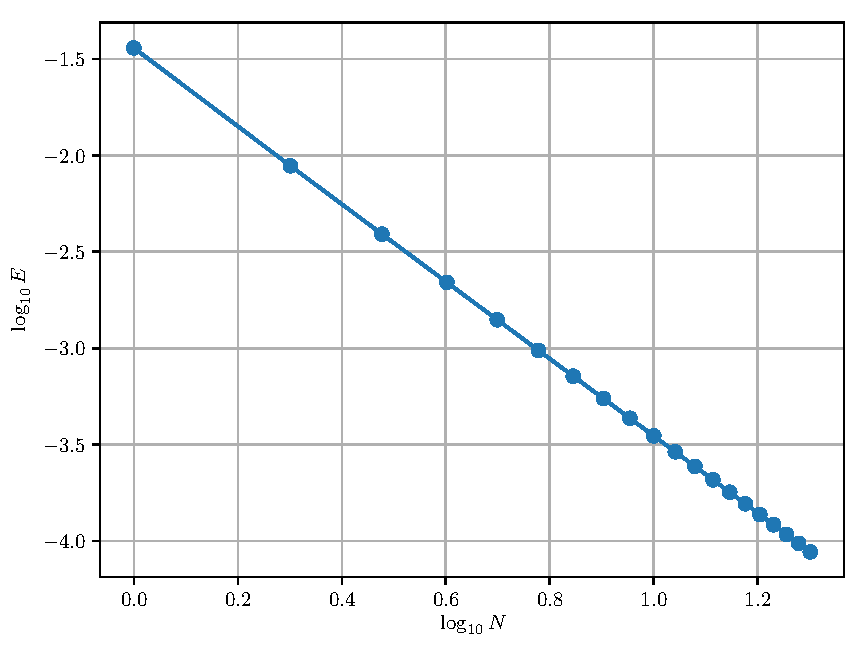
\includegraphics[width=\columnwidth]{plots/q4a.pdf}
		\caption
		{Logarithmic plot of the error E versus number of intervals N for $f(x) = \cos x$.}
		\label{fig:q4a}
	\end{figure}
	
	\subsection{Log Integration}
	
	The integral $I$ to be evaluated is shown in \cref{eq:log_x_integral}.
	
	\begin{equation} \label{eq:log_x_integral}
		I = \int\limits_{0}^{1} \log_e x dx 
	\end{equation}
	
	Using \cref{eq:context_total_integral} for $f(x) = \log_e x$, we obtain the integral shown in \cref{eq:log_total_integral}.
	
	\begin{equation} \label{eq:log_total_integral}
		I \approx \frac{1}{N} \sum_{i=0}^{N-1} \log_e \left[ \frac{1}{N} \left(i + \frac{1}{2} \right) \right]
	\end{equation}
	
	The actual value of the integral to which the estimation is compared is shown in \cref{eq:log_actual_integral}.
	
	\begin{equation} \label{eq:log_actual_integral}
		\int\limits_{0}^{1} \log_e x dx = -1
	\end{equation}
	
	The integral of $\log_e x$ is computed in the \code{q4.py} script shown in \cref{lst:q4}, with output shown in \cref{lst:q4_log}. The logarithmic plot of the error versus N can be seen in \cref{fig:q4b}. The straight-line slope of the plot is indicative of the fact that first-order Gauss-Legendre integration was used.
	
	\begin{figure}[!htb]
		\centering
		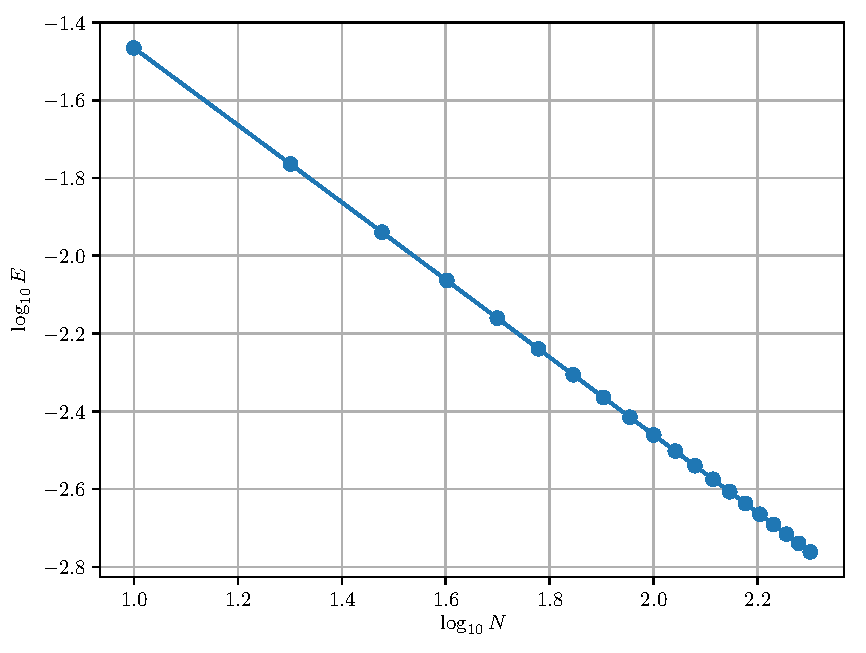
\includegraphics[width=\columnwidth]{plots/q4b.pdf}
		\caption
		{Logarithmic plot of the error E versus number of intervals N for $f(x) = \log_e x$.}
		\label{fig:q4b}
	\end{figure}
	
	\subsection{Log Integration Improvement}
	
	To have arbitrary interval widths, \cref{eq:total_integral} must be adjusted, as shown in \cref{eq:log_zeta_integral}, where $h_i$ is the width of interval $i$.
	
	\begin{equation} \label{eq:log_zeta_integral}
		I \approx \sum_{i=0}^{N-1} h_i f(x_{0_i}) 
	\end{equation}
	
	The relative widths used are shown in \cref{eq:relative_widths}.
	
	\begin{equation} \label{eq:relative_widths}
		(h_{rel_i})_{i=0}^{N-1} = (1, 2, 3, 4, 5, 6, 7, 8, 9, 10)
	\end{equation}
	
	These relative widths are converted to actual widths and then used to compute the integral in the \code{gauss\_legendre.py} script shown in \cref{lst:gauss_legendre}. The code is executed in the \code{q4.py} script shown in \cref{lst:q4}, with output shown in \cref{lst:q4_log}.	How closely the widths approximate the $\log_e x$ curve can be seen in \cref{fig:q4c}. The estimated value of the integral is $-0.988377$ with absolute error of $0.011622$. This is much more accurate than the equal-segment version in part (b), which obtained a value of $-0.965759$ and error of $0.034241$.
	
	\begin{figure}[!htb]
		\centering
		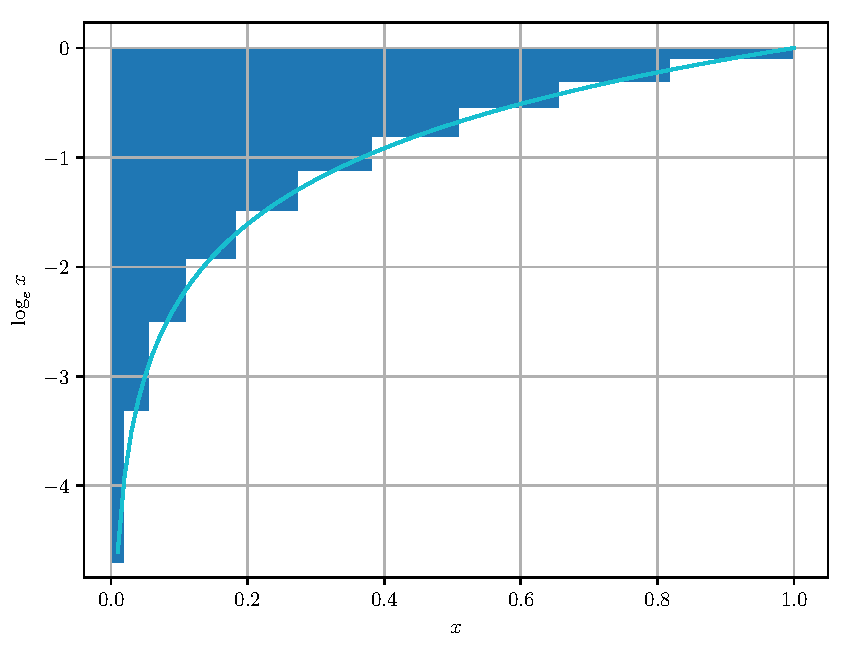
\includegraphics[width=\columnwidth]{plots/q4c.pdf}
		\caption
		{Sizes of intervals used for Question 4(c), with $\log_e x$ shown as reference.}
		\label{fig:q4c}
	\end{figure}

	\onecolumn
	
	\begin{appendices}
		
		\section{Code Listings} \label{appendix:code}
		
		\setminted{linenos,breaklines,fontsize=\footnotesize}
		
		\begin{center}
			\captionof{listing}{Custom matrix package (\texttt{matrices.py}).}
			\inputminted{python}{../matrices.py}
			\label{lst:matrices}
		\end{center}
	
		\begin{center}
			\captionof{listing}{Question 1 (\texttt{q1.py}).}
			\inputminted{python}{../q1.py}
			\label{lst:q1}
		\end{center}
	
		\begin{center}
			\captionof{listing}{Custom polynomial class (\texttt{polynomial.py}).}
			\inputminted{python}{../polynomial.py}
			\label{lst:polynomial}
		\end{center}
	
		\begin{center}
			\captionof{listing}{Tests of the custom polynomial class (\texttt{test\_polynomial.py}).}
			\inputminted{python}{../test_polynomial.py}
			\label{lst:test_polynomial}
		\end{center}
	
		\begin{center}
			\captionof{listing}{Lagrange interpolation (\texttt{lagrange.py}).}
			\inputminted{python}{../lagrange.py}
			\label{lst:lagrange}
		\end{center}
	
		\begin{center}
			\captionof{listing}{Tests of the Lagrange interpolation (\texttt{test\_lagrange.py}).}
			\inputminted{python}{../test_lagrange.py}
			\label{lst:test_lagrange}
		\end{center}
	
		\begin{center}
			\captionof{listing}{Question 2 (\texttt{q2.py}).}
			\inputminted{python}{../q2.py}
			\label{lst:q2}
		\end{center}
	
		\begin{center}
			\captionof{listing}{Newton-Raphson (\texttt{newton\_raphson.py}).}
			\inputminted{python}{../newton_raphson.py}
			\label{lst:newton_raphson}
		\end{center}
	
		\begin{center}
			\captionof{listing}{Piecewise-linear interpolation (\texttt{piecewise\_linear.py}).}
			\inputminted{python}{../piecewise_linear.py}
			\label{lst:piecewise_linear}
		\end{center}
	
		\begin{center}
			\captionof{listing}{Slope interpolation (\texttt{slope\_interpolation.py}).}
			\inputminted{python}{../slope_interpolation.py}
			\label{lst:slope_interpolation}
		\end{center}
	
	
		\begin{center}
			\captionof{listing}{Piecewise-linear interpolation tests (\texttt{test\_piecewise\_linear.py}).}
			\inputminted{python}{../test_piecewise_linear.py}
			\label{lst:test_piecewise_linear}
		\end{center}
		
		\begin{center}
			\captionof{listing}{Slope interpolation tests (\texttt{test\_slope\_interpolation.py}).}
			\inputminted{python}{../test_slope_interpolation.py}
			\label{lst:test_slope_interpolation}
		\end{center}
		
		\begin{center}
			\captionof{listing}{Question 3 (\texttt{q3.py}).}
			\inputminted{python}{../q3.py}
			\label{lst:q3}
		\end{center}
	
		\begin{center}
			\captionof{listing}{Newton-Raphson (\texttt{newton\_raphson\_matrix.py}).}
			\inputminted{python}{../newton_raphson_matrix.py}
			\label{lst:newton_raphson_matrix}
		\end{center}

		\begin{center}
			\captionof{listing}{Question 4 (\texttt{q4.py}).}
			\inputminted{python}{../q4.py}
			\label{lst:q4}
		\end{center}

		\begin{center}
			\captionof{listing}{Gauss-Legendre integration (\texttt{gauss\_legendre.py}).}
			\inputminted{python}{../gauss_legendre.py}
			\label{lst:gauss_legendre}
		\end{center}	
		\section{Output Logs} \label{appendix:logs}
		
		\begin{center}
			\captionof{listing}{Output of Question 1 program (\texttt{q1.txt}).}
			\inputminted{pycon}{logs/q1.txt}
			\label{lst:q1_log}
		\end{center}
	
		\begin{center}
			\captionof{listing}{Output of Question 2 program (\texttt{q2.txt}).}
			\inputminted{pycon}{logs/q2.txt}
			\label{lst:q2_log}
		\end{center}
	
		\begin{center}
			\captionof{listing}{Output of Question 3 program (\texttt{q3.txt}).}
			\inputminted{pycon}{logs/q3.txt}
			\label{lst:q3_log}
		\end{center}
	
		\begin{center}
			\captionof{listing}{Output of Question 4 program (\texttt{q4.txt}).}
			\inputminted{pycon}{logs/q4.txt}
			\label{lst:q4_log}
		\end{center}

	\end{appendices}

\end{document}
